\documentclass[12pt]{article}

\usepackage{enumitem}
\usepackage{booktabs}
\usepackage{graphicx}
\usepackage{caption}
\usepackage{subcaption}
\usepackage{float} % Para o uso do specifier [H]

\title{Especificação de Requisitos de Software para ProfScore}
\author{Carlos Henrique Cruz Xavier 
  \and Guilherme Vasconcelos Horita
  \and Leonardo Sousa Ferreira Fadul
}
\date{\today}

\begin{document}

\maketitle

\section{Introdução}

  \subsection{Propósito do documento de requisitos}

  O objetivo do projeto é criar um aplicativo que permita a avaliação dos professores universitários pelos alunos da UNIFEI.
  Este projeto destina-se aos alunos da Universidade Federal de Itajubá que estão em período de matrícula nas disciplinas.

  \subsection{Escopo do produto}

  O produto é um aplicativo que permite aos alunos da UNIFEI avaliar os professores com base em critérios pré-definidos, como metodologia, clareza, assiduidade, e outros aspectos relevantes.
  O aplicativo fornecerá relatórios de avaliação que poderão ser usados pela universidade para aprimorar o processo de ensino.
  O produto não incluirá funcionalidades como matrícula de alunos, gestão de notas, ou integração com outros sistemas acadêmicos.

  \subsection{Definições, acrônimos e abreviações}

  \begin{description}[leftmargin=*, widest=DCCHTM]
    
    \item[App]
    Aplicativo móvel ou web
    
    \item[DR]
    Documento de Requisitos

    \item[ProfScore]
    Professor Score
    
    \item[UNIFEI]
    Universidade Federal de Itajubá

    \item[Usuário]
    Aluno de universidade que utiliza o aplicativo

  \end{description}

  \subsection{Referências}

  \begin{itemize}
    \item IEEE Std 830-1998: \textit{IEEE Recommended Practice for Software Requirements Specifications}.
    \item Artigo ``Best Practices in Software Requirement Specifications'', John Doe, 2022, \textit{Journal of Software Engineering}.
  \end{itemize}

  \subsection{Visão geral do documento de requisitos}

  Este documento está organizado da seguinte maneira:
  \begin{itemize}
    \item \textbf{Descrição Geral} - Fornece uma visão geral do sistema, incluindo suas funcionalidades principais e restrições.
    \item \textbf{Requisitos Específicos} - Detalha os requisitos funcionais e não funcionais do sistema.
    \item \textbf{Modelos e Diagramação} - Apresenta diagramas de casos de uso, sequência e outros relevantes.
  \end{itemize}

  \section{Descrição Geral}
  \subsection{Perspectiva do Produto}
  \begin{itemize}
      \item \textbf{Usuário:} Alunos avaliam professores; administradores acessam relatórios detalhados.
      \item \textbf{Hardware:} Acessível por dispositivos desktop e móveis; hospedado em servidores.
      \item \textbf{Software:} A decidir.
      \item \textbf{Comunicação:} API RESTful para interação entre frontend e backend; notificações para usuários.
  \end{itemize}
  \subsection{Funções do Produto}
  Mostrar ranking dos professores de universidades e suas avaliações.
  \subsection{Características do Usuário}
  Alunos da UNIFEI.
  \subsection{Restrições}
  O software não será integrado com o sistema da UNIFEI.
  \subsection{Suposições e Dependências}
  \begin{itemize}
      \item Sistema Linux 
      \item ... 
  \end{itemize}
  
  \section{Requisitos Específicos}
  \subsection{Requisitos Não Funcionais}
      \subsubsection{RNF01 - Desempenho}
          O sistema deve ser capaz de suportar simultaneamente pelo menos 1.000 usuários ativos sem degradação significativa de desempenho.
      \subsubsection{RNF02 - Segurança}
          Todos os dados sensíveis devem ser criptografados tanto em trânsito quanto em repouso para garantir a segurança e a privacidade das informações dos usuários.
      \subsubsection{RNF04 - Usabilidade}
          O aplicativo deve ter uma interface intuitiva e responsiva, garantindo uma experiência de usuário satisfatória em dispositivos desktop e móveis.
      \subsubsection{RNF05 - Manutenibilidade}
          O código deve ser modular e bem documentado, facilitando a manutenção e a adição de novas funcionalidades.
  \subsection{ Interfaces Externas}
  \subsection{Requisitos Funcionais}
      \subsubsection{RF01 - Cadastro de Usuário}
          O sistema deve permitir o cadastro de novos usuários (alunos e administradores) com informações básicas como nome, e-mail e senha.
      \subsubsection{RF02 - Login e Autenticação}
          O sistema deve fornecer um mecanismo de autenticação seguro para que os usuários possam acessar o aplicativo com suas credenciais.
      \subsubsection{RF03 - Avaliação de Professores}
          Os alunos devem poder avaliar professores com base em critérios pré-definidos, como metodologia, clareza, assiduidade, etc.
      \subsubsection{RF04 - Visualização de Avaliações}
           Os alunos devem poder visualizar suas avaliações submetidas e o status atual das mesmas.
      \subsubsection{RF05 - Relatórios para Administradores}
          O sistema deve gerar relatórios detalhados das avaliações para os administradores da universidade, permitindo a análise das métricas.
      \subsubsection{RF06 - Gestão de Perfis}
          Usuários (alunos e administradores) devem poder atualizar suas informações de perfil, como e-mail e senha.
      \subsubsection{RF07 - Notificações}
          O sistema deve enviar notificações aos usuários sobre o status de suas avaliações e relatórios disponíveis.
      \subsubsection{RF08 - Filtro e Pesquisa de Professores}
          O sistema deve permitir que os alunos filtrem e pesquisem professores com base em critérios como departamento, nome e disciplinas lecionadas.
      \subsubsection{RF09 - Histórico de Avaliações}
          O sistema deve manter um histórico das avaliações realizadas por cada aluno, permitindo que eles revisitem e editem avaliações anteriores, se necessário, dentro de um período definido.
      \subsubsection{RF10 - Feedback e Sugestões}
          O sistema deve fornecer uma opção para que os alunos deixem feedback adicional e sugestões sobre os professores, além dos critérios de avaliação padrão. Este feedback será enviado para revisão e possível inclusão nos relatórios administrativos.
  
  \subsection{Requisitos Lógicos de Banco de Dados}
  \subsection{Restrições de Projeto}
  \subsection{Atributos do Sistema de Software}

  \newpage
  \section{Diagramas}
  \subsection{Caso de Uso}
  \begin{figure}[h]
  \centering
  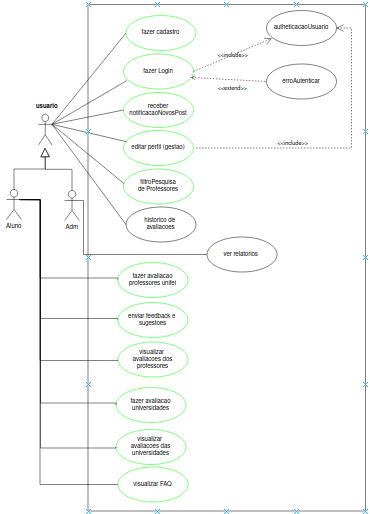
\includegraphics[width=1\textwidth]{diagramas/diag-casos-de-uso.png} % Insere uma imagem chamada diagrama.png
  \caption{Diagramas de Casos de Uso}
  \end{figure}
  % \clearpage
  
  % \subsection{Interação}
  % \begin{figure}[h]
  % \centering
  % 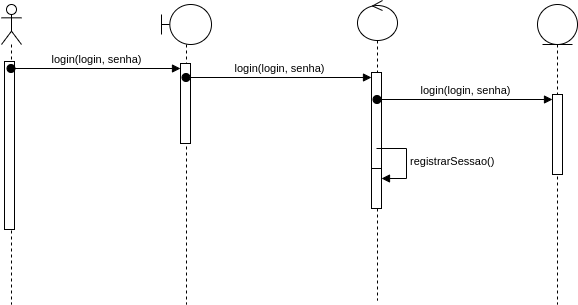
\includegraphics[width=1\textwidth]{imgs/diagramaInteracao.drawio.png} % Insere uma imagem chamada diagrama.png
  % \caption{Diagramas de Casos de Uso}
  % \end{figure}

  \subsection{Casos de Uso}

  % Please add the following required packages to your document preamble:
  % \usepackage{booktabs}
  \begin{table}[htbp]
    \caption{Caso de Uso para Cadastro de Usuário}
    \label{tab:cad-usuario}
    \resizebox{\textwidth}{!}{%
    \begin{tabular}{|c|c|}
    \hline
    \textbf{Nome Caso de Uso}                                          & Cadastro de Usuário                                                                          \\ \hline
    \textbf{Atores}                                                    & Aluno, Administrador                                                                         \\ \hline
    \textbf{Resumo}                                                    & O usuário se cadastra no sistema fornecendo nome, e-mail e senha.                            \\ \hline
    \textbf{Pré-condições}                                             & O usuário não deve estar previamente cadastrado no sistema.                                  \\ \hline
    \textbf{Pós-condições}                                             & O usuário é cadastrado e pode acessar o sistema utilizando suas credenciais.                 \\ \hline
    \textbf{Ação do Autor}                                             & \textbf{Ações do Sistema}                                                                    \\ \hline
    O ator preenche o formulário de cadastro com nome, e-mail e senha. &                                                                                              \\ \hline
                                      & O sistema valida os dados.                                                                   \\ \hline
                                      & Se válido, armazena as informações no banco de dados.                                        \\ \hline
    \textbf{}                                                          & Retorna uma confirmação de cadastro ao usuário.                                              \\ \hline
    \textbf{Restrição / Validação}                                     & O e-mail deve ser válido e único. A senha deve atender aos critérios de segurança definidos. \\ \hline
    \end{tabular}
    }
  \end{table}

  \begin{table}[htbp]
    \caption{Caso de Uso para Login e Autenticação}
    \label{tab:login-autent}
    \resizebox{\textwidth}{!}{%
    \begin{tabular}{|c|c|}
    \hline
    \textbf{Nome Caso de Uso} & Login e Autenticação \\ \hline
    \textbf{Atores} & Aluno, Administrador \\ \hline
    \textbf{Resumo} & O usuário realiza login no sistema utilizando e-mail e senha. \\ \hline
    \textbf{Pré-condições} & O usuário deve estar previamente cadastrado no sistema. \\ \hline
    \textbf{Pós-condições} & O usuário é autenticado e tem acesso às funcionalidades do sistema conforme seu perfil. \\ \hline
    \textbf{Ação do Autor} & \textbf{Ações do Sistema} \\ \hline
    O ator insere o e-mail e a senha no formulário de login. & O sistema valida as credenciais. \\ \hline
    & Se válidas, autentica o usuário e o redireciona para a página inicial. \\ \hline
    & Se inválidas, exibe uma mensagem de erro. \\ \hline
    \textbf{Restrição / Validação} & O sistema deve proteger as credenciais usando criptografia. \\ \hline
    \end{tabular}
    }
\end{table}

\begin{table}[htbp]
  \caption{Caso de Uso para Avaliação de Professores}
  \label{tab:avaliacao-prof}
  \resizebox{\textwidth}{!}{%
  \begin{tabular}{|c|c|}
  \hline
  \textbf{Nome Caso de Uso} & Avaliação de Professores \\ \hline
  \textbf{Atores} & Aluno \\ \hline
  \textbf{Resumo} & O aluno avalia professores com base em critérios predefinidos. \\ \hline
  \textbf{Pré-condições} & O aluno deve estar autenticado e ter cursado a disciplina do professor a ser avaliado. \\ \hline
  \textbf{Pós-condições} & A avaliação é registrada no sistema e pode ser visualizada posteriormente. \\ \hline
  \textbf{Ação do Autor} & \textbf{Ações do Sistema} \\ \hline
  O aluno acessa a página de avaliação do professor. & O sistema exibe os critérios de avaliação. \\ \hline
  O aluno preenche a avaliação com base nos critérios apresentados. & O sistema armazena a avaliação no banco de dados. \\ \hline
  & O sistema verifica se o aluno está autorizado a avaliar (cursou a disciplina). \\ \hline
  \textbf{Restrição / Validação} & O aluno só pode avaliar professores das disciplinas que cursou e dentro de um período definido. \\ \hline
  \end{tabular}
  }
\end{table}

\begin{table}[htbp]
  \caption{Caso de Uso para Visualização de Avaliações}
  \label{tab:visualizacao-avaliacoes}
  \resizebox{\textwidth}{!}{%
  \begin{tabular}{|c|c|}
  \hline
  \textbf{Nome Caso de Uso} & Visualização de Avaliações \\ \hline
  \textbf{Atores} & Aluno \\ \hline
  \textbf{Resumo} & O aluno visualiza as avaliações que submeteu e verifica seu status. \\ \hline
  \textbf{Pré-condições} & O aluno deve estar autenticado e ter avaliações previamente submetidas. \\ \hline
  \textbf{Pós-condições} & As avaliações submetidas pelo aluno são exibidas na tela. \\ \hline
  \textbf{Ação do Autor} & \textbf{Ações do Sistema} \\ \hline
  O aluno acessa a página de visualização de avaliações. & O sistema recupera as avaliações do banco de dados. \\ \hline
  & Exibe as avaliações e seus status ao aluno. \\ \hline
  \textbf{Restrição / Validação} & Apenas o aluno que submeteu a avaliação pode visualizá-la. \\ \hline
  \end{tabular}
  }
\end{table}

\begin{table}[htbp]
  \caption{Caso de Uso para Relatórios para Administradores}
  \label{tab:relatorios-admin}
  \resizebox{\textwidth}{!}{%
  \begin{tabular}{|c|c|}
  \hline
  \textbf{Nome Caso de Uso} & Relatórios para Administradores \\ \hline
  \textbf{Atores} & Administrador \\ \hline
  \textbf{Resumo} & O administrador gera relatórios detalhados das avaliações dos professores. \\ \hline
  \textbf{Pré-condições} & O administrador deve estar autenticado no sistema. \\ \hline
  \textbf{Pós-condições} & O relatório é gerado e pode ser visualizado ou exportado. \\ \hline
  \textbf{Ação do Autor} & \textbf{Ações do Sistema} \\ \hline
  O administrador solicita a geração de um relatório de avaliações. & O sistema gera o relatório com as métricas solicitadas. \\ \hline
  & Exibe o relatório ao administrador. \\ \hline
  & Permite a exportação do relatório, se necessário. \\ \hline
  \textbf{Restrição / Validação} & O acesso aos relatórios deve ser restrito a administradores. \\ \hline
  \end{tabular}
  }
\end{table}

\begin{table}[htbp]
  \caption{Caso de Uso para Gestão de Perfis}
  \label{tab:gestao-perfis}
  \resizebox{\textwidth}{!}{%
  \begin{tabular}{|c|c|}
  \hline
  \textbf{Nome Caso de Uso} & Gestão de Perfis \\ \hline
  \textbf{Atores} & Alunos, Administradores \\ \hline
  \textbf{Resumo} & Usuários podem atualizar informações de perfil, como e-mail e senha. \\ \hline
  \textbf{Pré-condições} & Usuário autenticado. \\ \hline
  \textbf{Pós-condições} & Informações de perfil atualizadas. \\ \hline
  \textbf{Ação do Autor} & \textbf{Ações do Sistema} \\ \hline
  1. Usuário acessa a seção de perfil. & 1. Sistema valida as informações inseridas. \\ \hline
  2. Atualiza informações de e-mail ou senha. & 2. Atualiza o perfil no banco de dados. \\ \hline
  3. Confirma as alterações. & 3. Confirma a atualização ao usuário. \\ \hline
  \textbf{Restrição / Validação} & 1. Senha deve atender a critérios de segurança (ex.: mínimo de caracteres, combinação de caracteres). \\ \hline
  \end{tabular}
  }
\end{table}

\begin{table}[htbp]
  \caption{Caso de Uso para Notificações}
  \label{tab:notificacoes}
  \resizebox{\textwidth}{!}{%
  \begin{tabular}{|c|c|}
  \hline
  \textbf{Nome Caso de Uso} & Notificações \\ \hline
  \textbf{Atores} & Alunos, Administradores \\ \hline
  \textbf{Resumo} & Sistema envia notificações sobre o status de avaliações e relatórios disponíveis. \\ \hline
  \textbf{Pré-condições} & Avaliações ou relatórios pendentes ou disponíveis. \\ \hline
  \textbf{Pós-condições} & Usuário notificado sobre status de avaliações e relatórios. \\ \hline
  \textbf{Ação do Autor} & \textbf{Ações do Sistema} \\ \hline
  1. Aluno/administrador realiza uma ação que altera o status de uma avaliação ou relatório. & 1. Sistema verifica mudanças no status de avaliações ou relatórios. \\ \hline
  & 2. Envia notificações ao usuário relevante. \\ \hline
  \textbf{Restrição / Validação} & As notificações devem ser enviadas apenas aos usuários afetados pelas mudanças de status. \\ \hline
  \end{tabular}
  }
\end{table}

\begin{table}[htbp]
  \caption{Caso de Uso para Filtro e Pesquisa de Professores}
  \label{tab:filtro-pesquisa-professores}
  \resizebox{\textwidth}{!}{%
  \begin{tabular}{|c|c|}
  \hline
  \textbf{Nome Caso de Uso} & Filtro e Pesquisa de Professores \\ \hline
  \textbf{Atores} & Alunos \\ \hline
  \textbf{Resumo} & Sistema permite filtrar e pesquisar professores por critérios como departamento, nome, e disciplinas lecionadas. \\ \hline
  \textbf{Pré-condições} & Usuário autenticado e acessando o módulo de busca. \\ \hline
  \textbf{Pós-condições} & Professores filtrados e exibidos conforme critérios. \\ \hline
  \textbf{Ação do Autor} & \textbf{Ações do Sistema} \\ \hline
  1. Usuário acessa a página de pesquisa de professores. & 1. Sistema exibe os critérios de filtragem disponíveis. \\ \hline
  2. Aplica filtros e realiza a busca. & 2. Realiza a busca conforme os critérios e exibe os resultados. \\ \hline
  \textbf{Restrição / Validação} & Pesquisa deve permitir combinações de critérios (ex.: departamento + nome). \\ \hline
  \end{tabular}
  }
\end{table}

\begin{table}[htbp]
  \caption{Caso de Uso para Histórico de Avaliações}
  \label{tab:historico-avaliacoes}
  \resizebox{\textwidth}{!}{%
  \begin{tabular}{|c|c|}
  \hline
  \textbf{Nome Caso de Uso} & Histórico de Avaliações \\ \hline
  \textbf{Atores} & Alunos \\ \hline
  \textbf{Resumo} & Sistema mantém um histórico das avaliações realizadas, permitindo edição dentro de um período definido. \\ \hline
  \textbf{Pré-condições} & Avaliações realizadas anteriormente. \\ \hline
  \textbf{Pós-condições} & Histórico atualizado com as edições feitas. \\ \hline
  \textbf{Ação do Autor} & \textbf{Ações do Sistema} \\ \hline
  1. Usuário acessa seu histórico de avaliações. & 1. Sistema exibe o histórico de avaliações. \\ \hline
  2. Revisa e edita avaliações dentro do prazo permitido. & 2. Permite a edição de avaliações dentro do período permitido. \\ \hline
  \textbf{Restrição / Validação} & Edição permitida apenas dentro de um período definido após a avaliação inicial. \\ \hline
  \end{tabular}
  }
\end{table}

\begin{table}[htbp]
  \caption{Caso de Uso para Feedback e Sugestões}
  \label{tab:feedback-sugestoes}
  \resizebox{\textwidth}{!}{%
  \begin{tabular}{|c|c|}
  \hline
  \textbf{Nome Caso de Uso} & Feedback e Sugestões \\ \hline
  \textbf{Atores} & Alunos \\ \hline
  \textbf{Resumo} & Sistema oferece opção para feedback adicional e sugestões sobre professores, enviado para revisão. \\ \hline
  \textbf{Pré-condições} & Usuário autenticado e já ter realizado uma avaliação. \\ \hline
  \textbf{Pós-condições} & Feedback e sugestões enviados para revisão e possível inclusão em relatórios administrativos. \\ \hline
  \textbf{Ação do Autor} & \textbf{Ações do Sistema} \\ \hline
  1. Usuário acessa a opção de feedback. & 1. Sistema recebe e armazena o feedback. \\ \hline
  2. Preenche feedback adicional e sugestões. & 2. Encaminha o feedback para revisão. \\ \hline
  3. Envia feedback. & 3. Sistema confirma o envio ao usuário. \\ \hline
  \textbf{Restrição / Validação} & Feedback deve ser validado para conteúdo adequado antes de ser enviado para revisão. \\ \hline
  \end{tabular}
  }
\end{table}

\begin{table}[htbp]
  \caption{Caso de Uso para Avaliar Universidade} 
  \label{tab:avaliarUniversidade} 
  \resizebox{\textwidth}{!}{% 
  \begin{tabular}{|c|c|} 
  \hline 
  \textbf{Nome Caso de Uso} & Avaliar Universidade \\ \hline 
  \textbf{Atores} & Alunos \\ \hline 
  \textbf{Resumo} & Sistema permite que os alunos avaliem uma universidade com base em vários critérios, como infraestrutura e qualidade acadêmica. \\ \hline 
  \textbf{Pré-condições} & Usuário autenticado e ter acesso à universidade a ser avaliada. \\ \hline 
  \textbf{Pós-condições} & Avaliação armazenada e disponível para revisão administrativa. \\ \hline 
  \textbf{Ação do Autor} & \textbf{Ações do Sistema} \ \hline
  
  1. Usuário acessa a opção de avaliar uma universidade. & 1. Sistema apresenta formulário de avaliação. \\ \hline
  2. Preenche os critérios de avaliação (ex.: infraestrutura, professores, etc.). & 2. Sistema valida e armazena a avaliação. \\ \hline
  3. Envia avaliação. & 3. Sistema confirma o envio ao usuário e disponibiliza para análise. \\ \hline 
  \textbf{Restrição / Validação} & Avaliação deve seguir diretrizes de conteúdo adequado. \\ \hline 
  \end{tabular} } 
\end{table}

\begin{table}[htbp]
  \caption{Caso de Uso para Filtro e Pesquisa de Universidade}
  \label{tab:filtro-pesquisa-universidade}
  \resizebox{\textwidth}{!}{%
  \begin{tabular}{|c|c|}
  \hline
  \textbf{Nome Caso de Uso} & Filtro e Pesquisa de Universidade \\ \hline
  \textbf{Atores} & Alunos \\ \hline
  \textbf{Resumo} & Sistema permite que os alunos filtrem e pesquisem universidades com base em critérios como localização, curso oferecido, e avaliação geral. \\ \hline
  \textbf{Pré-condições} & Usuário autenticado. \\ \hline
  \textbf{Pós-condições} & Exibição de universidades filtradas de acordo com os critérios estabelecidos. \\ \hline
  \textbf{Ação do Autor} & \textbf{Ações do Sistema} \\ \hline
  1. Usuário acessa a opção de pesquisa de universidades. & 1. Sistema apresenta campos de filtro e pesquisa. \\ \hline
  2. Define os critérios de filtro (ex.: localidade, curso). & 2. Sistema busca universidades com base nos critérios fornecidos. \\ \hline
  3. Executa a pesquisa. & 3. Sistema exibe os resultados filtrados. \\ \hline
  \textbf{Restrição / Validação} & Universidades devem atender aos critérios de pesquisa inseridos pelo usuário. \\ \hline
  \end{tabular}%
  }
\end{table}

\begin{table}[htbp]
  \caption{Caso de Uso para Visualizar FAQ}
  \label{tab:visualizar-faq}
  \resizebox{\textwidth}{!}{%
  \begin{tabular}{|c|c|}
  \hline
  \textbf{Nome Caso de Uso} & Visualizar FAQ \\ \hline
  \textbf{Atores} & Alunos \\ \hline
  \textbf{Resumo} & Sistema exibe uma lista de perguntas frequentes (FAQ) para os alunos, proporcionando respostas rápidas para dúvidas comuns. \\ \hline
  \textbf{Pré-condições} & Usuário autenticado. \\ \hline
  \textbf{Pós-condições} & Perguntas frequentes são exibidas de acordo com o tema selecionado. \\ \hline
  \textbf{Ação do Autor} & \textbf{Ações do Sistema} \\ \hline
  1. Usuário acessa a opção de visualização de FAQ. & 1. Sistema exibe a lista de perguntas frequentes disponíveis. \\ \hline
  2. Visualiza as perguntas e respostas disponíveis. & 2. Sistema permite que o usuário selecione e visualize as respostas para cada pergunta. \\ \hline
  \textbf{Restrição / Validação} & As perguntas frequentes exibidas devem estar organizadas por categorias e seguir as políticas do sistema. \\ \hline
  \end{tabular}%
  }
\end{table}


\section{Diagramas de Sequência}

\begin{figure}[H] % Alterado para [H] para forçar o posicionamento
    \centering
    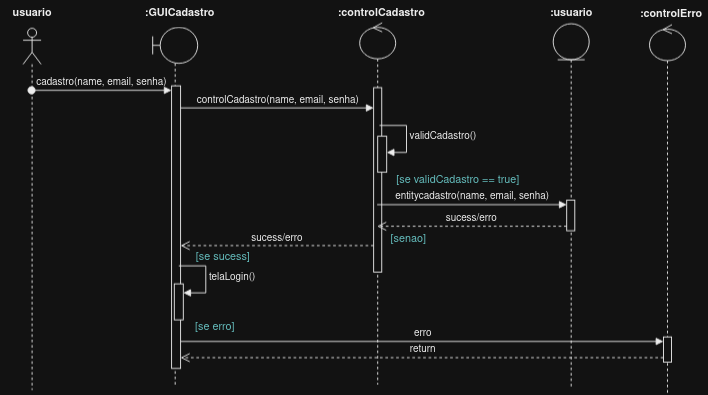
\includegraphics[width=0.8\textwidth]{diagramas/i1-cadastro-usuario.png}
    \caption{Cadastro de Usuário}
    \label{fig:i1-cadastro-usuario}
\end{figure}

\begin{figure}[H]
    \centering
    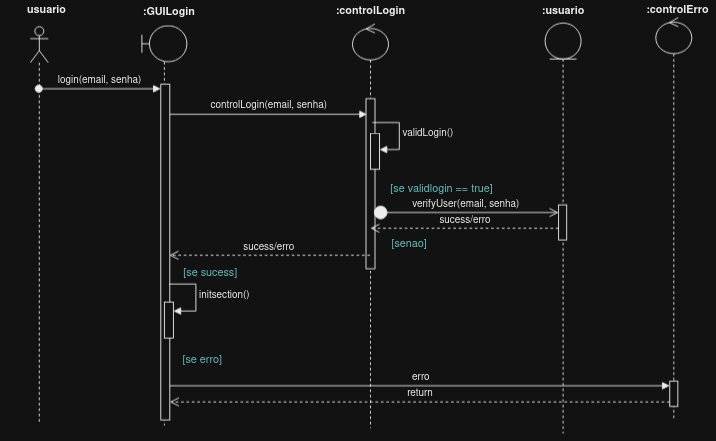
\includegraphics[width=0.8\textwidth]{diagramas/i2-login-autent.png}
    \caption{Login e Autenticação}
    \label{fig:i2-login-autent}
\end{figure}

\begin{figure}[H]
    \centering
    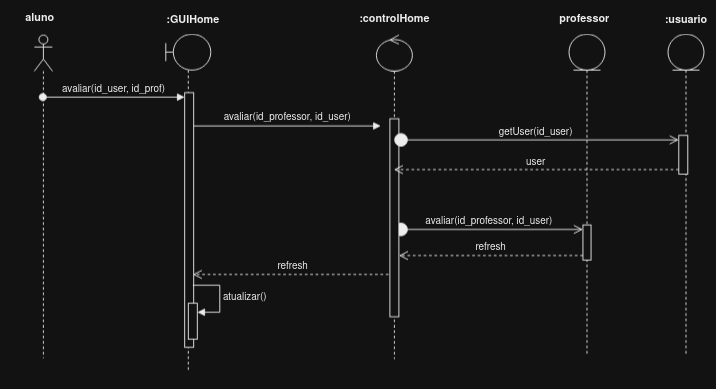
\includegraphics[width=0.8\textwidth]{diagramas/i3-avaliac-professores.png}
    \caption{Avaliação de Professores}
    \label{fig:i3-avaliac-professores}
\end{figure}

\begin{figure}[H]
    \centering
    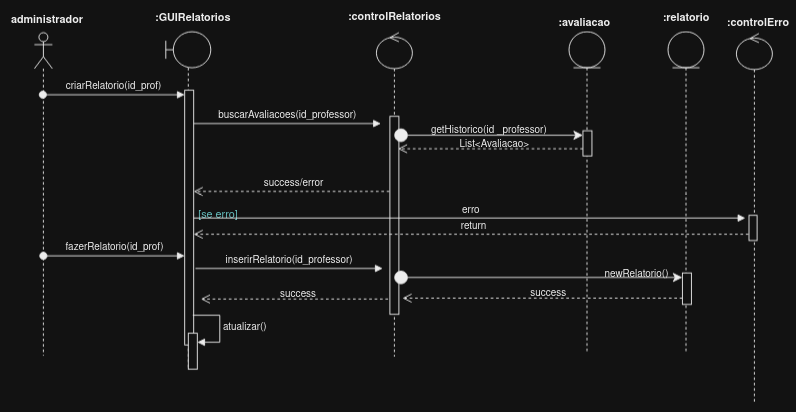
\includegraphics[width=0.8\textwidth]{diagramas/i5-relatorios-admin.png}
    \caption{Relatórios Administrativos}
    \label{fig:i5-relatorios-admin}
\end{figure}

\begin{figure}[H]
    \centering
    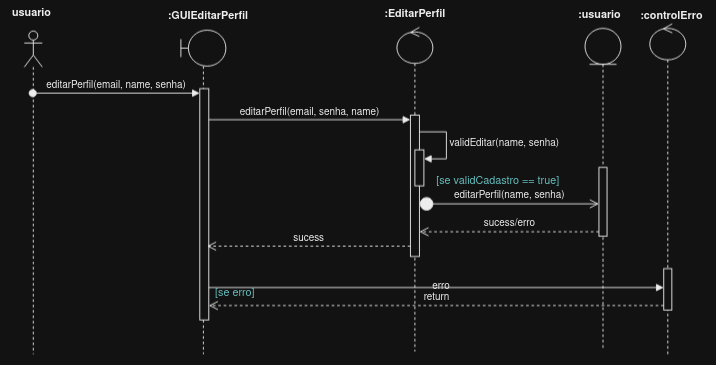
\includegraphics[width=0.8\textwidth]{diagramas/i6-gestao-editar-perfil.png}
    \caption{Gestão e Edição de Perfil}
    \label{fig:i6-gestao-editar-perfil}
\end{figure}

\begin{figure}[H]
    \centering
    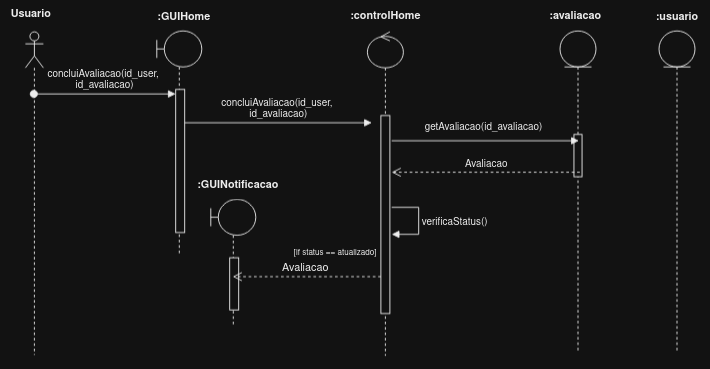
\includegraphics[width=0.8\textwidth]{diagramas/i7-enviar-notificacoes.png}
    \caption{Envio de Notificações}
    \label{fig:i7-enviar-notificacoes}
\end{figure}

\begin{figure}[H]
    \centering
    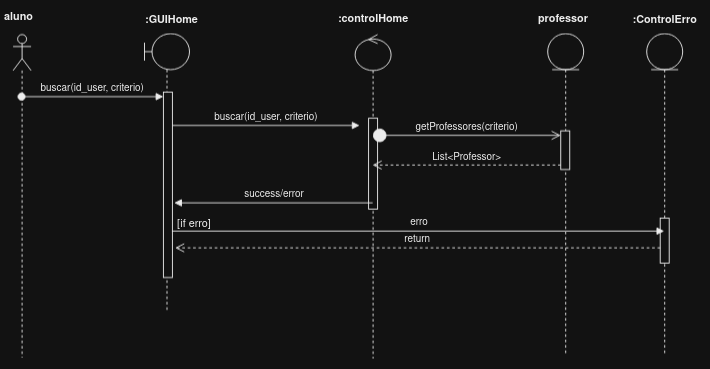
\includegraphics[width=0.8\textwidth]{diagramas/i8-filtro-pesq-professor.png}
    \caption{Filtro e Pesquisa de Professor}
    \label{fig:i8-filtro-pesq-professor}
\end{figure}

\begin{figure}[H]
    \centering
    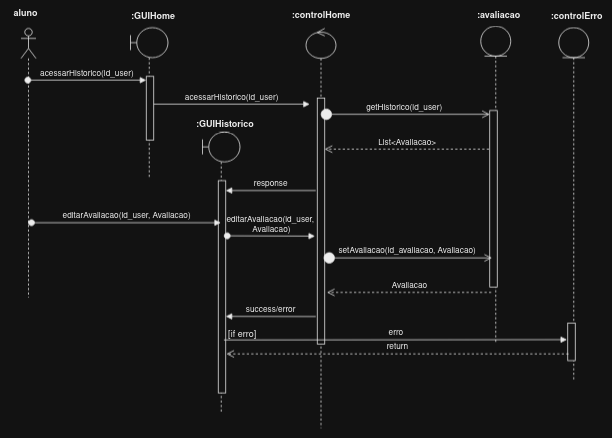
\includegraphics[width=0.8\textwidth]{diagramas/i9-historico-avaliacoes.png}
    \caption{Histórico de Avaliações}
    \label{fig:i9-historico-avaliacoes}
\end{figure}

\begin{figure}[H]
    \centering
    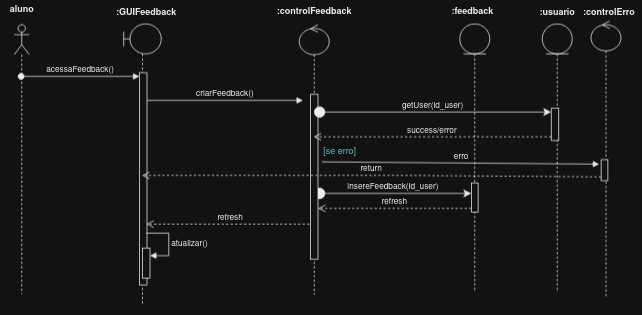
\includegraphics[width=0.8\textwidth]{diagramas/i10-feedback-sugestoes.png}
    \caption{Feedback e Sugestões}
    \label{fig:i10-feedback-sugestoes}
\end{figure}

\begin{figure}[H]
  \centering
  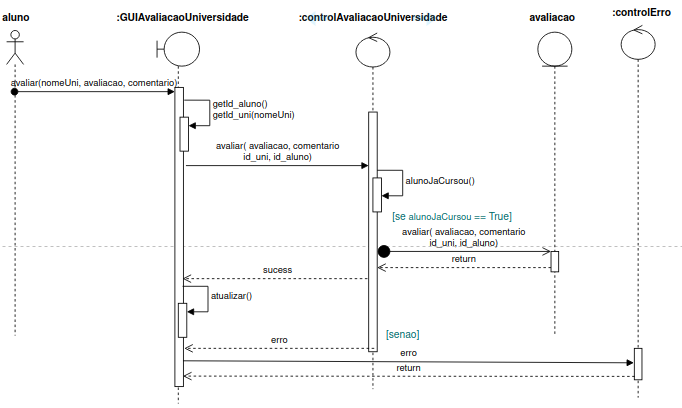
\includegraphics[width=0.8\textwidth]{diagramas/i11-avaliar-univ.png}
  \caption{Avaliar Universidade}
  \label{fig:i11-avaliar-univ}
\end{figure}

\begin{figure}[H]
  \centering
  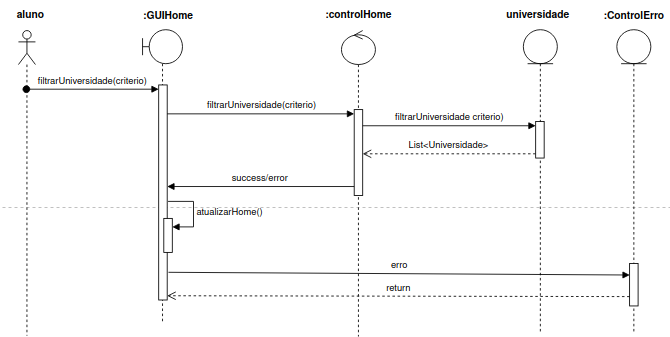
\includegraphics[width=0.8\textwidth]{diagramas/i12-filtro-pesq-univ.png}
  \caption{Filtro e Pesquisa de Universidade}
  \label{fig:i12-filtro-pesq-univ}
\end{figure}

\begin{figure}[H]
  \centering
  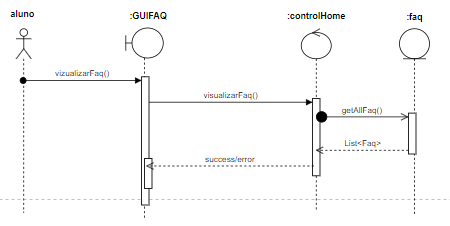
\includegraphics[width=0.8\textwidth]{diagramas/i13-visualizar-faq.png}
  \caption{Visualizar FAQ}
  \label{fig:i13-visual-faq}
\end{figure}

\section{Diagramas de Classes}

\begin{figure}[H] % Alterado para [H] para forçar o posicionamento
    \centering
    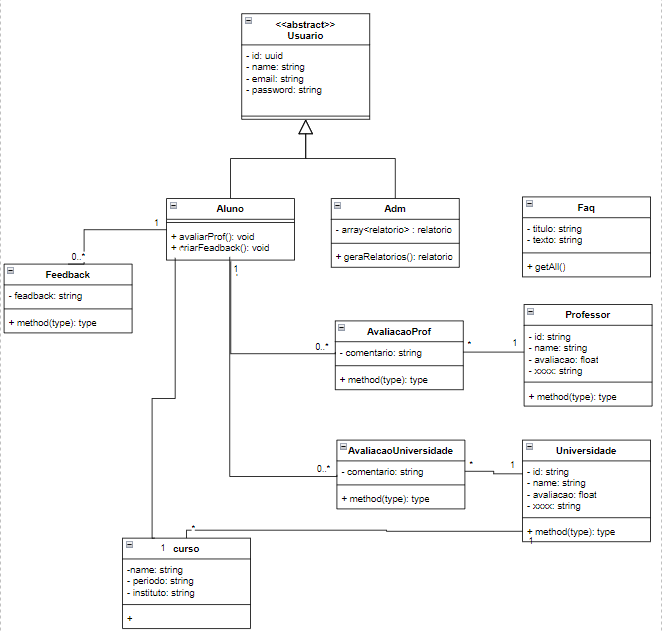
\includegraphics[width=0.8\textwidth]{diagramas/diag-classes-com-faq.png}
    \caption{Diagrama de classes do ProfScore}
    \label{fig:diag-classes}
\end{figure}

\section{Interfaces}

\begin{figure}[H] % Alterado para [H] para forçar o posicionamento
    \centering
    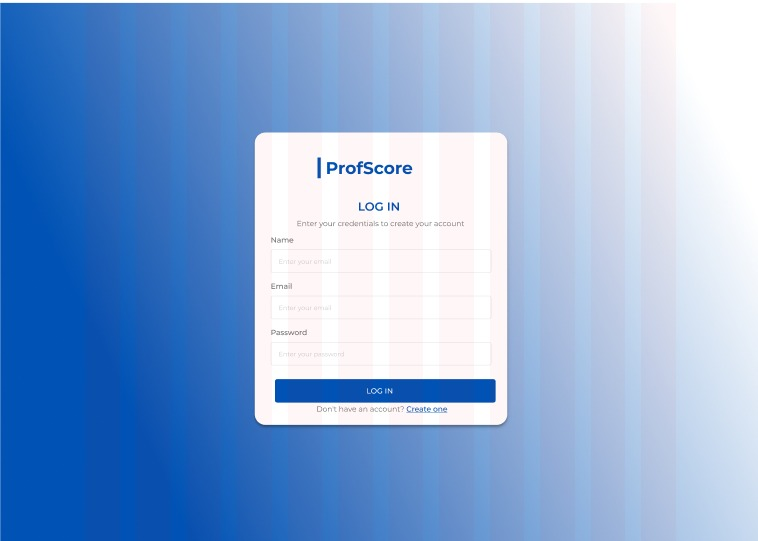
\includegraphics[width=0.8\textwidth]{interfaces/i1-login.png}
    \caption{Interface de Login}
    \label{fig:i1-login}
\end{figure}

\begin{figure}[H] % Alterado para [H] para forçar o posicionamento
  \centering
  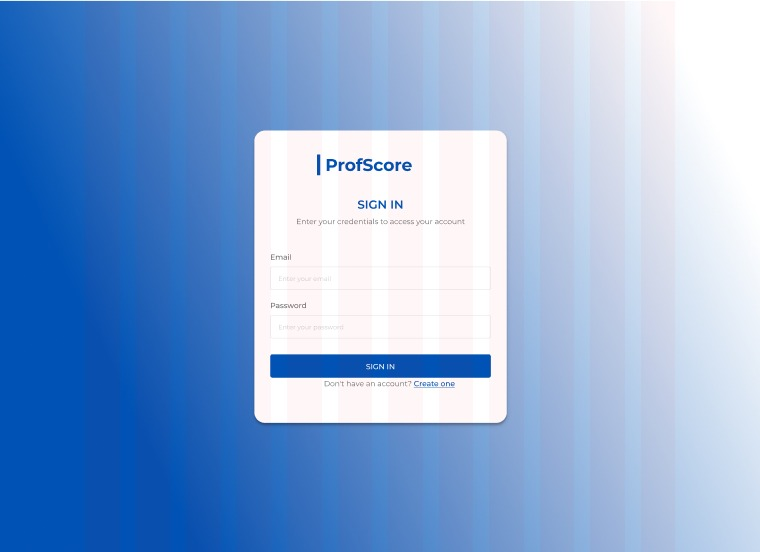
\includegraphics[width=0.8\textwidth]{interfaces/i2-signin.png}
  \caption{Interface de Sign Up}
  \label{fig:i2-signin}
\end{figure}

\begin{figure}[H] % Alterado para [H] para forçar o posicionamento
  \centering
  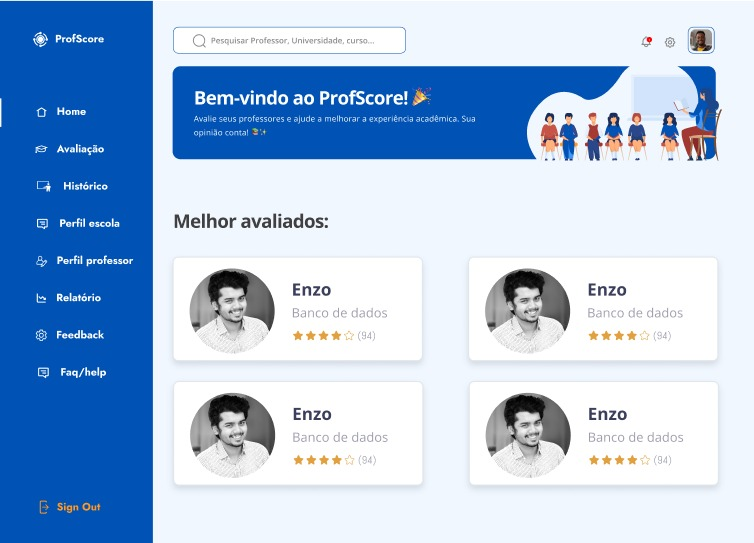
\includegraphics[width=0.8\textwidth]{interfaces/i3-home.png}
  \caption{Interface da Home Page}
  \label{fig:i3-home}
\end{figure}

\begin{figure}[H] % Alterado para [H] para forçar o posicionamento
  \centering
  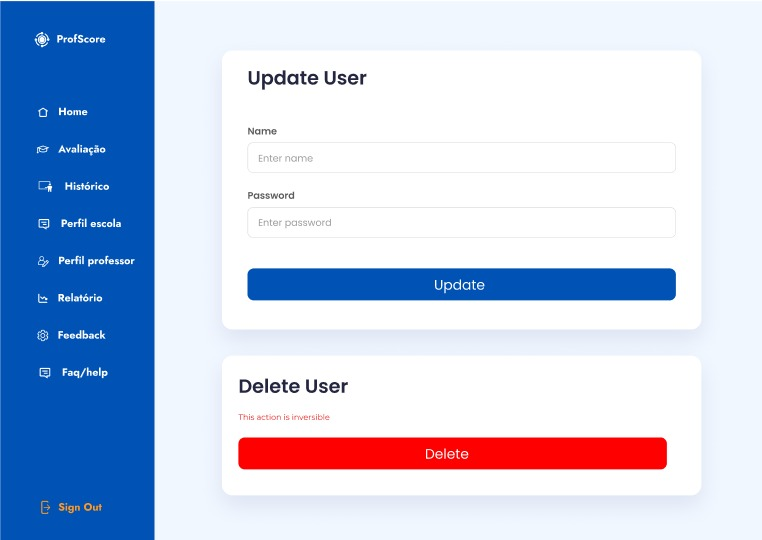
\includegraphics[width=0.8\textwidth]{interfaces/i4-update-user.png}
  \caption{Interface de Atualização de Usuário}
  \label{fig:i4-update-user}
\end{figure}

\begin{figure}[H] % Alterado para [H] para forçar o posicionamento
  \centering
  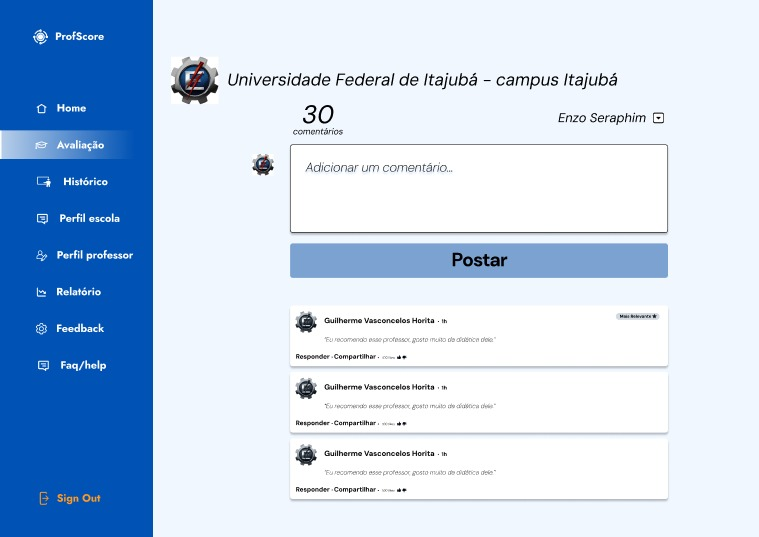
\includegraphics[width=0.8\textwidth]{interfaces/i5-avaliar-prof.png}
  \caption{Interface de Avaliação de Professor}
  \label{fig:i5-avaliar-prof}
\end{figure}

\begin{figure}[H] % Alterado para [H] para forçar o posicionamento
  \centering
  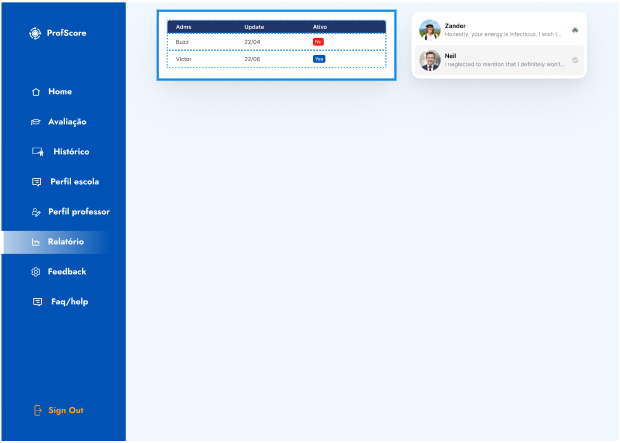
\includegraphics[width=0.8\textwidth]{interfaces/i6-relatorio.png}
  \caption{Interface dde Relatórios Administrativos}
  \label{fig:i6-relatorio}
\end{figure}

\begin{figure}[H] % Alterado para [H] para forçar o posicionamento
  \centering
  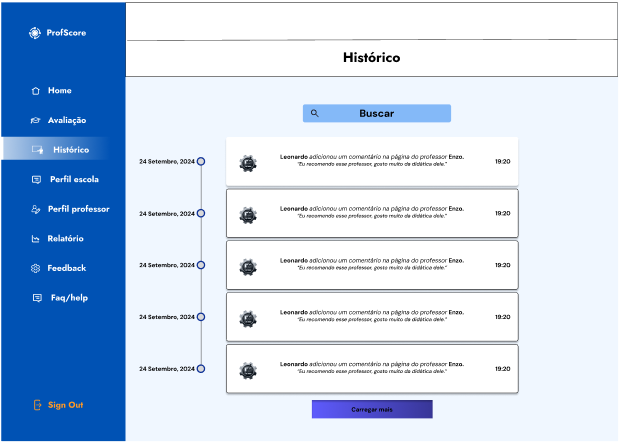
\includegraphics[width=0.8\textwidth]{interfaces/i7-historico.png}
  \caption{Interface de Histórico de Avaliações}
  \label{fig:i7-historico}
\end{figure}

\begin{figure}[H] % Alterado para [H] para forçar o posicionamento
  \centering
  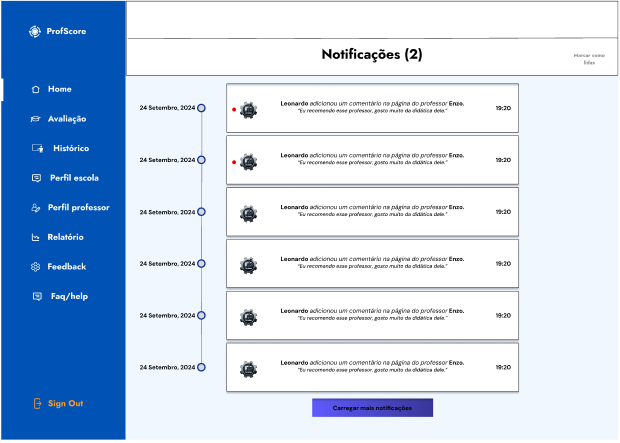
\includegraphics[width=0.8\textwidth]{interfaces/i8-notificacoes.png}
  \caption{Interface de Notificações}
  \label{fig:i8-notificacoes}
\end{figure}

\begin{figure}[H] % Alterado para [H] para forçar o posicionamento
  \centering
  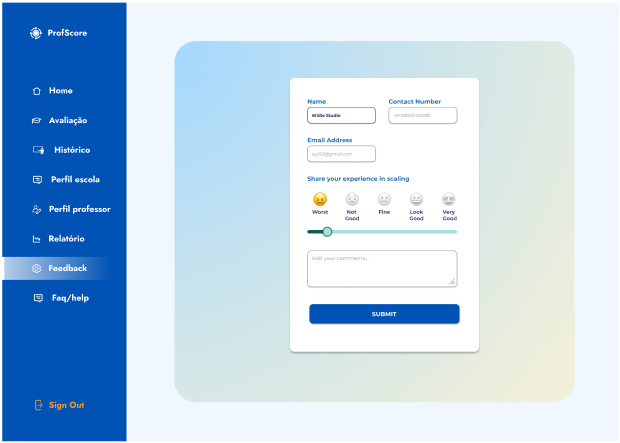
\includegraphics[width=0.8\textwidth]{interfaces/i9-feedback.png}
  \caption{Interface de Feedback e Sugestões}
  \label{fig:i9-feedback}
\end{figure}

\begin{figure}[H] % Alterado para [H] para forçar o posicionamento
  \centering
  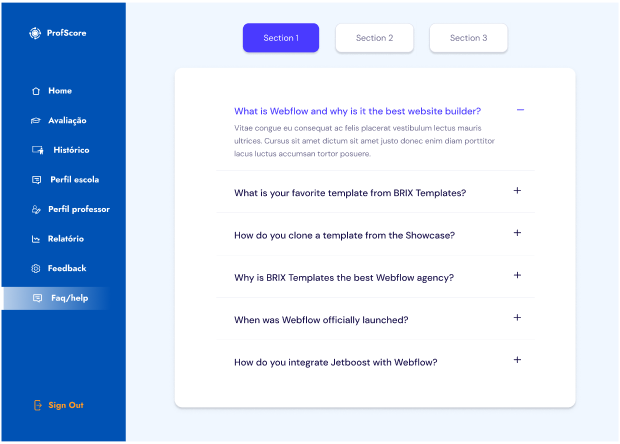
\includegraphics[width=0.8\textwidth]{interfaces/i10-faq.png}
  \caption{Interface de FAQ}
  \label{fig:i10-faq}
\end{figure}

\begin{figure}[H] % Alterado para [H] para forçar o posicionamento
  \centering
  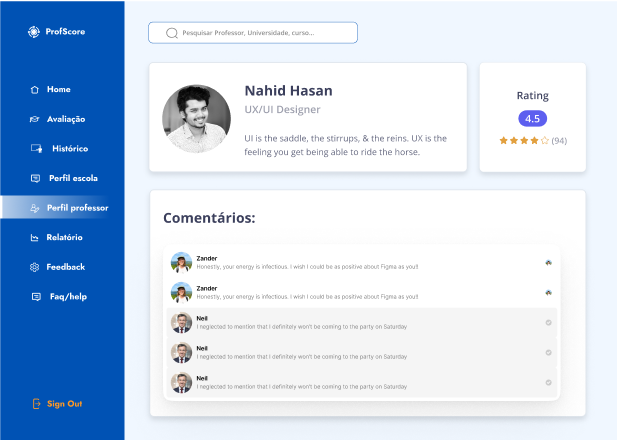
\includegraphics[width=0.8\textwidth]{interfaces/i11-perfil-prof.png}
  \caption{Interface de Perfil de Professor}
  \label{fig:i11-perfil-prof}
\end{figure}

\begin{figure}[H] % Alterado para [H] para forçar o posicionamento
  \centering
  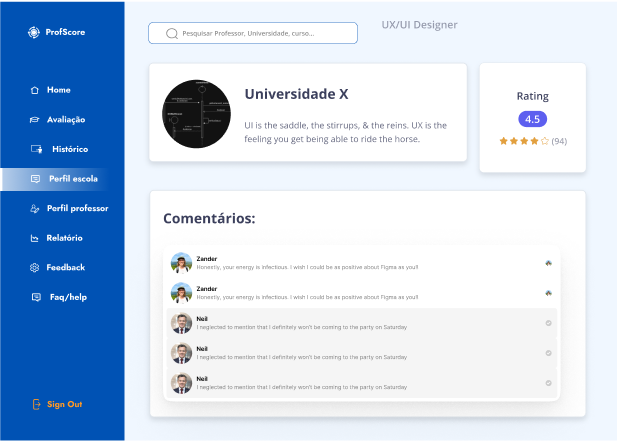
\includegraphics[width=0.8\textwidth]{interfaces/i12-perfil-univ.png}
  \caption{Interface de Perfil de Universidade}
  \label{fig:i12-perfil-univ}
\end{figure}

\end{document}